% \documentclass[12pt, letterpaper]{article}  % change to >11 pt if you like, and change article with report


\RequirePackage{fix-cm}
\documentclass[12pt, oneside]{report}
\usepackage[fontsize=12pt]{scrextend}
\usepackage[utf8]{inputenc}
\usepackage[letterpaper]{geometry}

\newenvironment{asbtract}{}{}
\usepackage{abstract}
\usepackage{listings} %to insert code listings
\usepackage[table,x11names]{xcolor}
\usepackage{stackengine}
% \newlength\llength
% \llength=1.38ex\relax

\usepackage{textcomp} % to write angular brackets with \textlangle

\definecolor{codegreen}{rgb}{0,0.6,0}
\definecolor{codegray}{rgb}{0.5,0.5,0.5}
\definecolor{codepurple}{rgb}{0.58,0,0.82}
\definecolor{backcolour}{rgb}{0.95,0.95,0.92}
\lstdefinestyle{mystyle}{
    backgroundcolor=\color{backcolour},   
    commentstyle=\color{codegreen},
    keywordstyle=\color{magenta},
    numberstyle=\tiny\color{codegray},
    stringstyle=\color{codepurple},
    basicstyle=\ttfamily\footnotesize,
    breakatwhitespace=false,         
    breaklines=true,                 
    captionpos=b,                    
    keepspaces=true,                 
    numbers=left,                    
    numbersep=5pt,                  
    showspaces=false,                
    showstringspaces=false,
    showtabs=false,                  
    tabsize=2
}
\lstset{columns=flexible}

% To define figures, listings, tables, etc with section counting
\usepackage{chngcntr}
\counterwithin{figure}{section}
\AtBeginDocument{\counterwithin{lstlisting}{section}}

\usepackage{titling}
\usepackage[backend=biber, sorting=none]{biblatex}
\usepackage{changepage}
\usepackage{lastpage} %info sul # dell'ultima pagina del documento
\usepackage{fancyhdr} %per modificare dimensioni,margini, intestazioni e righe a piè di pagina


\usepackage{tabularx} % to build flexible tables
\usepackage{array}
\usepackage{array,booktabs}% http://ctan.org/pkg/{array,booktabs}

\usepackage{makecell, caption, chngcntr} %
\usepackage{subcaption}

\usepackage{graphicx}
\graphicspath{/home/federico/Downloads/tesi}
\usepackage{color}
\usepackage{graphbox}
\usepackage[colorlinks=true]{hyperref}

\usepackage[]{todonotes}
%\usepackage[disable]{todonotes}
\newcommand{\td}[1]{\todo[inline]{#1}}

\usepackage{siunitx} % used for scientific notation like 1e-10
\sisetup{output-exponent-marker=\ensuremath{\mathrm{e}}}
\usepackage{float}
\usepackage{bm}
\usepackage{layouts}
\usepackage{lipsum}


\newcommand{\hr}[2]{\hyperref[#1]{\textbf{#2 \ref{#1}}}}
\newcommand{\ttt}[1]{\texttt{#1}}
\newcommand{\subtitle}[1]{%
  \posttitle{%
    \par\end{center}
    \begin{center}\large#1\end{center}
    \vskip0.5em}%
}
\newcommand\setrow[1]{\gdef\rowmac{#1}#1\ignorespaces}
\newcommand\clearrow{\global\let\rowmac\relax}
\clearrow
\newcolumntype{P}[1]{>{\centering\arraybackslash}p{#1}}

\definecolor{Maroon}{cmyk}{0, 0.87, 0.68, 0.32}
\usepackage[colorlinks=true]{hyperref}
\hypersetup{
    colorlinks=true,
    citecolor=black,
    filecolor=black,
    linkcolor=black, % colore dei link interni
    urlcolor=Maroon  % colore dei link interniesterni
}


\fancypagestyle{plain}{
  % cancella tutti i campi di intestazione e piè di pagina
  \fancyhf{}
  
  \cfoot{Page \thepage{} of \pageref{LastPage}} %es: pag: 4 di 10

  %linea orizzontale alle posizioni top e bottom della pagina
  \renewcommand{\headrulewidth}{0 pt}  
  \renewcommand{\footrulewidth}{0 pt}
}

\pagestyle{plain} 
\addbibresource{mybib.bib}

\title{\vspace{-2cm}\textbf{A multi-protocol communication layer for FastFlow's distributed runtime}}
% \subtitle{\textbf{An analysis}}
\author{
    \normalsize{\textbf{Federico Finocchio} - 516818}\\
    \normalsize{MSCS: Data and Knowledge. \underline{f.finocchio@studenti.unipi.it}}\\\\
}

\makeatletter
\renewenvironment{abstract}{%
    \if@twocolumn
      \section*{\abstractname}%
    \else %% <- here I've removed \small
      \begin{center}%
        {\bfseries \normalsize\abstractname\vspace{\z@}}%  %% <- here I've added \Large
      \end{center}%
      \quotation
    \fi}
    {\if@twocolumn\else\endquotation\fi}
\makeatother

\setcounter{tocdepth}{1}

\begin{document}
\date{}
\maketitle
    
\begin{abstract}
\normalsize
Handling the explosion in data production rates both for scientific and commercial applications require amount of storage and computational power which can't be handled in single machines, thus a shift to distributed computing is being recorded. This shift in programming environment requires new tools and frameworks, as well as new abstractions, to allow application developers to provide efficient applications which deal with real-time decisions in an accurate and actionable way.

FastFlow framework provides a set of abstraction that targets both the application and RTS developer, allowing via structured parallel programming the development of efficient parallel applications via a compositional model based on LEGO-style building blocks. In this work we introduce a new abstraction at the communication layer, allowing to connect remote nodes via a multitude of transports in different parts of the FastFlow application, allowing heterogeneity in computing nodes.
\end{abstract}
\tableofcontents
\newpage
\chapter*{Introduction}
\label{introduction}
%todo aggiustare numbering delle reference. Exa-big viene messa 8 ma in realtà dovrebbe essere la prima visto che la uso in intro ora
\addcontentsline{toc}{section}{\nameref{introduction}}
In the past years we are experiencing an explosion in the quantities of produced data, coming from scientific simulations, experimental facilities, connected devices (IoT) and commercial applications. These huge amount of data challenge, the storage and computing capabilities of single machines as well the network being used to transfer data between multiple machines due to I/O bottleneck \cite{exa-big}. Moreover, the amount of computation needed to handle the necessary data for modern applications, like (near) real-time applications that generate near-continuous data, is much bigger than the one offered by current monolithic systems. Thus, as we witnessed the shift from sequential to parallel programming, we are now observing a new shift from parallel to distributed computing. Moreover, as the difference between Big Data and High Performance Computing becomes more and more blurred, and due to this new evolution in the way application are developed and deployed, new frameworks, programming models and tools have surfaced to help the programmer to deal with the complexity of designing parallel applications above the underlying distributed infrastructures \cite{exa-big, survey-distributed}. In the transition to distributed computing, new extensive parallel processing and new analytics algorithms are needed in order to provide timely and actionable information \cite{big-data-movingforward}. However, dealing with scalable and parallel applications that can be deployed across the network is not an easy task, and abstractions are needed in order to allow the application developers to focus on the optimization of the uppermost layer, leaving, among all, communication and synchronization details to experts on the respective fields.

The shift towards distributed computing introduces new challenges, like resource management, data distribution, coordination of participating processes and monitoring of the application. Given that each of these challenges acts at a different abstraction layer, application developers often prefer to rely over high-abstraction frameworks to abstract from the distributed challenges and focus only on the application development.\newline

The thesis aims at extending the existing distributed-memory runtime system for FastFlow, a C++ structured parallel programming library originally targeting shared-memory platforms. The thesis introduces a novel communication layer, which offers a standardized API in order to abstract from the underlying transport used for communications between remote nodes. The provided abstraction allows the \textit{application programmer} to design new applications, as well as extending existing ones, by leveraging the classes introduced in this work in order to connect different nodes on the network without having to deal with communication specific implementation. The implemented layer provides an automatized way of plugging different protocols inside existing application without breaking the code and with little to zero effort. The \textit{RTS programmer} is provided with a set of extensible classes in order to allow the integration of existing transports or even future ones. Furthermore, in order to follow and maintain the LEGO style \textit{philosophy} of the FastFlow library, also the implemented communication layer is composed of a set of building blocks which can be composed in order to address the needs of the specific application. Allowing composability of components is very important in heterogeneous environments such as the cloud, in order to allow easy porting of applications and adaptation to environment changes. To fulfill this need, the communication layer presented in this thesis allows each application subset to communicate using the protocol that is most suited for the task at hand or for the architecture specific limitations. Vendor specific transports can represent a limitation in horizontally scaling applications, in particular if the provided transports are completely \textit{obscure} to the application programmer, which should not care of the underlying communication aspects when programming a distributed application. The implemented building blocks allow for this reason to be run above a multitude of different transports by simply plugging the protocol-specific building block.\newline
%TODO quelli implementati da me non sono building blocks ma semplicemente dei nodi che verrano poi usati internamente in modo trasparente dall'utente. Quello che l'utente deve fare è semplicemente descrivere un json con tutte i protocolli che vuole usare ad un determinato step.
A natural preliminary phase of this work was strictly tied to the analysis of communication frameworks which are available to the application programmer in order to leverage efficiently multiple protocols during communication between distributed groups. We aim at building a communication layer which is agnostic of the underlying protocol, thus, we first implemented the communication classes by means of a multi-protocol RPC framework in order to enable communication between nodes in a protocol-agnostic fashion. In the first part of this work we analysed the Margo \cite{mochi-core} library, it's underlying RPC framework called Mercury \cite{mochi-core, mercury} and the threading library which is used by Margo as a runtime framework, called Argobots \cite{argobots-paper}. The three analyzed frameworks are part of a much broad set of frameworks which are referred to as \textit{Mochi core}, as specified in \cite{mochi-core}.  The Mochi core provides a set of frameworks to enable communication, concurrency management and storage with a composition model. As appeared by the testing we performed, but as also described by its developers, the Mercury RPC framework is purposefully built to leverage HPC fabrics vendor protocols, sometimes resulting in a lack of support and faulty implementation for more classical transports like MPI and TCP. This led us to adapt the existing MPI and TCP drivers in the distributed FastFlow RTS into the novel API. 

The thesis uses a bottom-up approach to illustrate the overall picture of the used frameworks and to describe internally each of those frameworks. The thesis is organized as follows:
\begin{itemize}
	\item \hr{chap:background}{Chapter}: illustrates the state-of-the-art regarding communication frameworks in the HPC and BDA environments;
	\item \hr{chap:fastflow}{Chapter}: presents the FastFlow library and its current stage of development, illustrates the distributed runtime which is further extended by this work;
    \item \hr{sec:mercury}{Chapter}: presents the core framework which provides the building blocks needed to implement RPC calls leveraging multiple transports. We describe the general structure of the framework, which will serve to describe the higher-level framework used to implement the communication layer in FastFlow's distributed runtime;
    \item \hr{sec:argobots}{Chapter}: describes the runtime system which is used by the higher-level RPC framework in order to manage concurrent execution of different RPCs, to allow asynchronous execution of RPC-related callbacks and to simplify Mercury's progress loop;
    \item \hr{sec:margo}{Chapter}: describes the high level framework used for the implementation of the multi-protocol interface for the communication layer in FastFlow's distributed runtime. We show how this framework leverages Mercury and Argobots functionalities to provide a parallel and efficient multi-protocol RPC framework;
    \item \hr{sec:implementation}{Chapter}: gives insights on the integration of Margo's functionalities into the FastFlow's distributed communication layer. We show pseudo-code of the implemented classes and common use-cases for both the application and runtime programmer;
    \item \hr{sec:testing}{Chapter}: focuses on the presentation of sample applications and testing we performed to evaluate the effectiveness of the implemented communication layer.
\end{itemize}

\section{Background}

\chapter{FastFlow}
\label{chap:fastflow}
FastFlow is the result of a joint effort of the Parallel Programming Model Group of the University of Pisa and the Parallel Computing Research Group of the University of Turin. FastFlow is a C++ structured parallel programming framework, that leverages a streaming data-flow approach and originally targeted cache-coherent shared-memory architectures \cite{fastflow}. It was recently extended with a distributed-memory runtime in order to allow developers to build and deploy FastFlow applications over distributed environments. The FastFlow library was built with a layered design by keeping efficiency in the base mechanisms to maintain efficiency across the whole framework \cite{fastflow-highlevel}. Each of the implemented layers provides abstractions at different levels in order to help both the application and the RTS developer. The top level abstractions provide classical parallel patterns targeting the application developer, the lowest layers instead expose abstractions for the RTS programmer, by providing a reduced set of \texttt{Building Blocks} (BBs from now on), that can be used to efficiently implement most of the existing parallel applications \cite{fastflow-highlevel}.

\section{Building Blocks}
\texttt{Building Block}s are the core elements of FastFlow programming, since they are used as the basic abstraction layer to properly build FastFlow streaming parallel patterns. \texttt{BB}s come in two flavor, \textit{sequential} and \textit{parallel} and they both rely over Single-Producer Single-Consumer (SPSC) lock-free queues to share memory and allow efficient communication.\newline

The implemented building-blocks are the \textit{pipeline}, \textit{farm} and the \textit{all-to-all}. The \textit{pipeline} building block has a double usage, in fact it can be used to connect building blocks and to build pipeline parallelism. The \textit{farm} is used to express functional replication which is controlled both in input and output by \texttt{Emitter} and \texttt{Collector} entities which can be specialized in order to implement different dispatching/gathering policies. Finally, the \textit{all-to-all} building block offers the possibility to implement the shuffle communication pattern and to remove bottlenecks coming from centralized entities in the \textit{farm} building block.

The main characteristic of \texttt{building blocks} is their composition-oriented nature, which allows the programmer to assemble them in a LEGO-style fashion in order to build complex parallel applications. This reflects the style of the structured parallel programming methodology and enables a more organized way to build parallel applications.

\section{FastFlow distributed runtime}
Since the last version of FastFlow, a distributed runtime has been added which allows for FastFlow applications to be organized and deployed over distributed computing nodes via a set of wrappers class and renewed \texttt{BB} components. The introduced mechanisms for the distributed runtime allows the programmer to easily and efficiently divide and deploy an existing application into \textit{distributed groups}, as well as creating a new application directly for the distributed environment retaining the same LEGO-style approach for parallel application on shared-memory systems.\newline

The distributed extension for the FastFlow library is provided by modification at the \texttt{BB} level in order to provide the easy porting of existing shared-memory FastFlow application into the distributed environment without dealing with the burden of handling distributed communications; provide a set of mechanisms to implement higher-level ready-to-use distributed patterns.
\subsection{Transition to distributed-memory}
The transition from shared-memory to distributed-memory required the creation of new concepts, as the one of \textit{distributed groups}, as well as new abstractions, as the classes for serialization and communication of the task to be sent across the network. Existing applications can be deployed in the distributed environment by retaining the semantic of the original FastFlow application. The only modifications required for an application programmer to transform a shared-memory FastFlow application into a mixed shared/distributed-memory application are related to the identification of disjoint \textit{distributed groups} via the provided API calls and the mapping of each group to an endpoint by means of a JSON configuration file.

The distributed groups (\textit{dgroups} henceforth) represent logical partitions of the original FastFlow application which are executed on remote nodes. Each one of the \textit{dgroups} is realized as a shared-memory application to fully exploit the potential of the single nodes. Moreover, the resulting \textit{dgroup} is internally plugged with specific sequential \texttt{BB}s and node wrappers to realize serialization/deserialization and communication between the deployed \textit{dgroups} by retaining the original application semantic.


\section{Mercury}
\label{sec:mercury}
Mercury \cite{mochi-core, mercury} is an asynchronous RPC framework purposefully built to efficiently provide communication services to HPC systems with high-performance fabrics. It provides an abstracted network implementation to enable transparent support to future systems and protocols, efficient use of existing native transport mechanisms, and support of large data arguments via the RDMA enabled interface. Moreover, it provides an asynchronous RPC interface, based on a callback system, that allows transfer of parameters and procedure calls in the context of both local and remote execution in order to completely remove the differentiation of communications between on and off-node.\newline

The library allows the execution of arbitrary functions via a system of function tagging and callbacks, coupled to a queue system that saves procedure calls which are pending and still not executed. The receiving process drives the progress loop in which arguments are retrieved, function calls are executed, and the results are sent back to the origin node.\newline

Additionally, the library offers the possibility of being ported to various systems since the network layer is abstracted and the application interface is based on a simple set of network primitives for both point-to-point messaging and one-sided RDMA. The network abstraction layer functionalities are implemented on top of different plugins. The plugin system can be considered as a \textit{compatibility} layer, which implements the communication functionalities offered by different protocols. Examples of plugins are Libfabric \cite{libfabric, ofi_plugin}, MPI \cite{mpi_plugin} and UCX \cite{openucx}, and multiple protocols are offered by each of the plugin, ranging from vendor-specific protocols to more classic ones like TCP and UDP.\newline

\subsection{RPC: a Mercury's perspective}
General RPC frameworks provide the possibility to serialize function parameters and ship them to a remote node that will execute the respective function call. As stated in \cite{mercury}, Mercury tries to address two main problems:
\begin{itemize}
    \item inability to take advantage of HPC high performance communication protocols: standard frameworks are usually designed on top of TCP/IP protocols, which represent a limitation over the performances often required by HPC systems;
    \item inability to transfer large amount of data: standard RPC frameworks doesn't allow (or discourage) transfer of large amount of data through the implemented mechanisms.
\end{itemize}

Mercury addresses these limitations by offering an asynchronous and flexible RPC interface specifically tailored for HPC systems. To do this, Mercury exposes an abstracted API to perform asynchronous RPC as well as large data transfer, and completely relies on the underlying network implementation provided by the plugins, in order to be independent from the used transport mechanism. As stated in \cite{mercury}, Mercury's main purpose is to serve as a basis for higher-level frameworks that need to remotely exchange data in a distributed environment, by offering a flexible interface completely decoupled from the underlying protocol and system specifications.

\subsection{Architecture}
Mercury is built on a two-layer architecture, as shown in \hr{fig:mercury-rpc-components}{Figure}, where each layer provides an abstraction for specific functionalities. The lowermost layer offers abstractions needed to provide networking functionalities such as point-to-point messaging, address lookup, remote memory access, progress and cancellation. The uppermost layer is further divided in two service-level components, referred to as \textit{RPC interface} and \textit{bulk data interface}. The RPC interface allows the programmer to remotely execute function calls, shipping function arguments and receiving results from the remote node; the bulk interface, instead, complements the RPC interface and allows large data transfer via the creation of memory descriptors, which enables the possibility to initiate raw memory transfers using remote memory access, whenever the underlying system provides it.\newline
\begin{figure}[H]
    \centering
    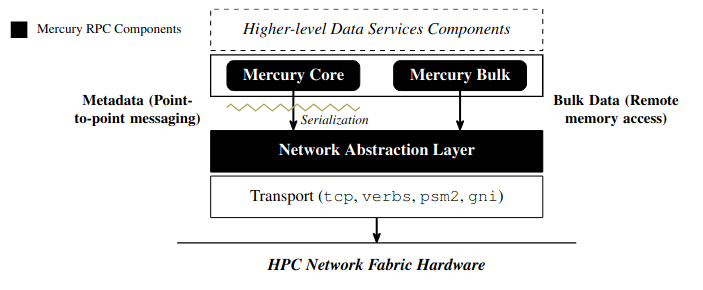
\includegraphics[width=0.8\linewidth]{res/RPC_components.png}
    \caption{Mercury RPC components in the software stack.}
    \label{fig:mercury-rpc-components}
\end{figure}

Mercury extends the functionalities of another project, called \textit{I/O Forwarding Scalability Layer} (IOFSL)\cite{iofsl}, which allows RPC calls specifically related to file-system-specific I/O operations. By extending this layer, Mercury allows to generate RPC calls to generic functions that can be dynamically defined and registered in the application using Mercury.

\subsubsection{Plugins}
\label{plugins}
The plugin functionalities are referred to as a ``\textit{support for various network protocols that can be easily added and selected at runtime}'' \cite{nal_guide}.
Given that Mercury's main aim is to leverage the high performance solutions provided by HPC network fabrics, which requires specific low-level vendor APIs, Mercury relies on plugins as an intermediate layer for network functionalities. In order to overcome the burden of implementing the network abstraction layer directly on top of those APIs, Mercury relies over various plugins for the implementation of functionalities like RDMA and point-to-point messaging. A multitude of plugins are provided by the framework, however the vast majority of them is under testing or being deprecated, leaving as ``stable'' only the ones related to Libfabric, UCX and shared-memory \cite{sm_plugin} for local nodes communication. We show in \S\ref{limitations} the main limitations we have encountered during testing of these plugins.\newline

Switching between various plugins is very simple and can be done by specifying a predefined string containing the desired plugin paired with the needed protocol to use during communications. Each plugin defines its own format, but common fields are shared among the configuration strings of various plugins, and they mostly refer to the type of plugin and the protocol to be used. Format of strings is provided in \hr{tab:mercury-string}{Table}.

\begingroup
\renewcommand{\arraystretch}{1.3} % Default value: 1
\begin{table}[H]
\begin{center}
    \begin{tabular}{ | c | c | c |}
    %\begin{adjustwidth}{0cm}{}
         \hline
         \textbf{Plugin} & \textbf{Protocol} & \textbf{Initialization format}\\ [0.5ex] 
         \hline\hline
         ofi & tcp & \text{ofi+tcp[://\textlangle{}hostname,IP,interface name\textrangle{}:\textlangle{}port\textrangle{}]}\\
         & verbs & ofi+verbs[://[domain/]\textlangle{}hostname,IP,interface name\textrangle{}:\textlangle{}port\textrangle{}]\\
         & psm2 & ofi+psm2\\
         & gni & ofi+gni[://\textlangle{}hostname,IP,interface name\textrangle{}]\\\hline
         ucx & all & ucx+all[://[net\_device/]\textlangle{}hostname,IP,interface name\textrangle{}:\textlangle{}port\textrangle{}]\\
         & tcp & ucx+tcp[://[net\_device/]\textlangle{}hostname,IP,interface name\textrangle{}:\textlangle{}port\textrangle{}]\\
         & rc,ud & ucx+\textlangle{}rc,ud\textrangle{}[://[net\_device/]\textlangle{}hostname,IP,interface name\textrangle{}:\textlangle{}port\textrangle{}]\\\hline
         na & sm & na+sm[://\textlangle{}shm\_prefix\textrangle{}]\\\hline
         mpi & dynamic, static & mpi+\textlangle{}dynamic, static\textrangle{}\\\hline
    \end{tabular}
    \caption{Mercury plugin's initialization format.}
    \label{tab:mercury-string}
    %\end{adjustwidth}
    \end{center}
\end{table}
\endgroup

Note, however, that plugins may behave differently regarding how the format string is provided, in fact plugins do not manage incomplete or incorrect configuration strings uniformly. Some of these issues are reported in \S\ref{limitations}.

\subsubsection{Network Abstraction Layer}
\label{sec:NAL}
The Network Abstraction Layer (NAL) provides an abstraction of the network infrastructure above which the communications are executed. It is a simple abstraction which only provides limited functionalities, like address lookup, point-to-point messaging, remote memory access, progress, and cancellation.\newline

The abstractions provided by this layer allows the uppermost layers to be completely agnostic of the underlying communication protocol implemented via the plugin system. Moreover, The API is non-blocking and uses a callback mechanism to provide asynchronous execution. Progress is driven by API calls which allows user callbacks to be placed in completion queue and retrieved for execution.\newline

Mercury refers to communicating nodes as \ttt{origin} and \ttt{target}, indicating respectively the node issuing the request and the node receiving it. Both origin and target nodes must specify the desired plugin/protocol pair at initialization phase, by providing a string as described in \S\ref{plugins}. Since a node can both provide and ask for services, the only time a server-specific behaviour is defined only refers to initialization, where the user can specify if the current node will be listening for incoming RPCs. Besides this, no more server/client concepts are used in the following.\newline

The functionalities offered by the NAL refers to three main mechanisms:
\begin{itemize}
    \item expected messages: requires a \textit{receive} operation to be pre-posted by the target. Therefore, this requires the origin node to be known in advance, before the receive operation is posted. If the receive operation is not posted before the message is sent, it can be dropped;
    \item unexpected messages: does not require the target to post a receive operation for the message, and they can arrive from any source. The target can retrieve received messages in an asynchronous way. These messages are allowed to be dropped, but the plugin can decide to queue them anyway;
    \item remote memory access: allows registration of memory chunks which can be later accessed by target nodes. Abstractions are provided through API which contains operations generally provided by most RDMA protocols.
\end{itemize}

The network abstraction is designed to allow emulation of one-sided operations, such as RDMA, on top of two-sided operations. In this way, Mercury can easily adapt to protocols which only supports fixed operations, like TCP/IP ones, where one-sided communications are not possible.


\subsubsection{RPC Layer}
The RPC layer allows nodes to issue remote calls, and it is based on the messaging model described in \S\ref{sec:NAL}. RPC requests are based on the common knowledge of origin and target nodes on how to encode and decode function parameters and return values.\newline
\begin{figure}[H]
    \centering
    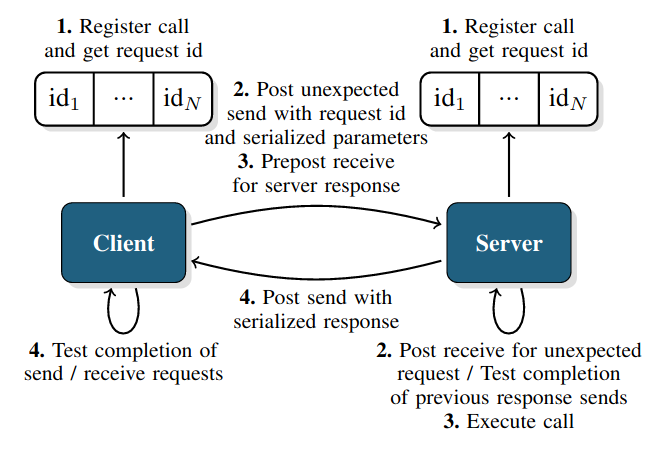
\includegraphics[width=0.6\linewidth]{res/rpc-flow.png}
    \caption{Execution flow of RPC call. }
    \label{fig:rpc-flow}
\end{figure}

Mercury provides mechanisms to support a set of generic function calls avoiding hard-coded routines. To allow this, origin and target nodes must register a unique function name along with encoding and decoding routines by using shared input/output types. We postpone the precise description of the registration process to \S\ref{sec:rpc-reg}, since Margo introduces few additional steps, which are the ones that are actually used to implement FastFlow's communication classes. We show in \hr{fig:rpc-flow}{Figure} a usual flow of execution needed by both origin and target nodes to execute a RPC request. The registered function is mapped to an ID which will be used in all the communications between the two nodes. A further step is needed by the target, which must register a callback that will be executed every time that ID is received. Once the functions are registered, the origin sends an \textit{unexpected} message to the target.\newline

Two situation may occur during an RPC request, and different mechanisms are used to guarantee full asynchrony:
\begin{itemize}
    \item the RPC call expects a response from the target: the origin node prepares its memory buffer to receive the response and uses the buffer to pre-posts an \textit{expected receive}. At the reception of the response, the origin node can retrieve the response from the callback queue and proceed;
    \item the RPC call does not expect a response from the target: the origin node, at the moment of RPC registration, declares that this RPC does not expect a response. An RPC of this kind allows the origin node to proceed without posting a receive operation, progress can be made as soon as the request is sent to the target.
\end{itemize}

From the target side, receiving an \textit{unexpected} message with a specified ID translates in the execution of the callback registered at startup by decoding the parameters sent by the origin, and sending the outputs by encoding them at the end of execution, if the registered RPC expects a response.
\subsubsection{Bulk Layer}
This layer allows to send large data by avoiding intermediate memory copies. It is performed by creating a local memory handle which points to previously registered areas of memory (not necessarily contiguous) which the target node can access via RDMA operations. The bulk layer is directly built on top of the RDMA interface defined in the network abstraction layer. \newline

\begin{figure}[H]
    \centering
    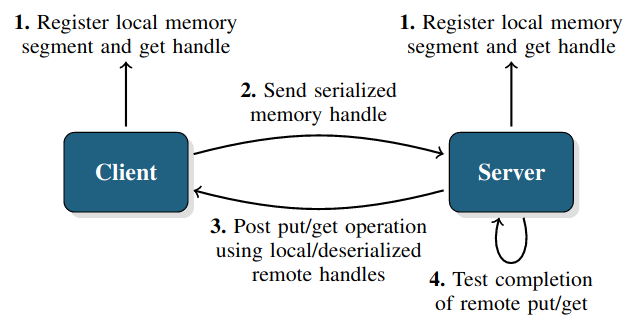
\includegraphics[width=0.6\linewidth]{res/bulk-flow.png}
    \caption{Execution flow of bulk request.}
    \label{fig:bulk-flow}
\end{figure}

A typical execution flow for a bulk request is depicted in \hr{fig:bulk-flow}{Figure}. The target node manages all the bulk transfers in order to be able to control the data flow and protect its memory from concurrent accesses. This operation is one-sided, and it is started by the origin node which creates a bulk data descriptor, serializes it, and send the serialized descriptor to the target as an argument via a specific RPC request. Once the descriptor has been deserialized by the target, two situations can occur. The request can be related to \textit{consumption} or \textit{production of data}. In both cases the target node creates a memory handle to manage the request, allocating the necessary memory. However, in the first case the target initiates a remote \texttt{read} operation before performing the function call, in the second case the target executes the call and initiates a remote \texttt{write} operation with the produced results.\newline

Memory handles are an important building block for memory transfer, in particular in such cases where non-contiguous memory is to be transferred. The memory of the communicating nodes is abstracted by the memory handle and allows to access memory in a transparent way without modifications to the process described above.

\subsection{Resilience and Fault Tolerance}
The fault tolerance mechanism is mainly provided by the possibility to interrupt calls and reclaim resources of pending operations after these have been signaled as \textit{cancelled}. Cancellation is an asynchronous and local operation. From a user perspective, completion of offloaded operations is known only when the associated callback is placed in the local queue of pending operations. When a callback is triggered and the operation was locally canceled by the user, that operation is reported as canceled and aborted.\newline

A basic flow of events related to the cancellation of an operation is shown in \hyperref[fig:op-cancel]{\textbf{Figure \ref{fig:op-cancel}}}.

\begin{figure}[H]
    \centering
    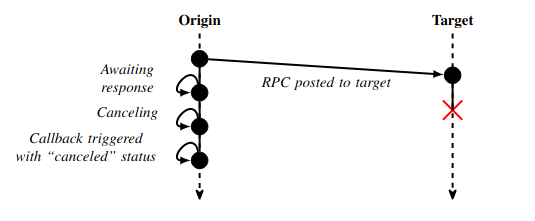
\includegraphics[width=0.6\linewidth]{res/op-cancel.png}
    \caption{Cancellation of an RPC operation.}
    \label{fig:op-cancel}
\end{figure}

\subsection{Dependencies}
As reported by \cite{merc_git}, the dependencies are mostly related to the intended plugin to integrate inside a specific application. No further requirements are specified by the Mercury's developers as needed for the installation and use of their framework.


\subsection{Mercury analysis}
\label{sec:mercury-analysis}
Mercury comes with lots of functionalities and drawbacks. We list in this section all the advantages and the main limitations of the Mercury framework encountered during the testing phase, which are therefore shared by all the higher-level libraries which are based on it.

\subsubsection{Advantages}
Mercury's interface allows to easily enable communication using a system of plugin which offers compatibility with a multitude of network and vendor specific protocols. The Mercury library, once again, shows the importance of having an abstraction layer to provide efficient use of underlying protocols without having a complete expertise on how they work. Being able to address different needs and to leverage the functionalities of different systems, by the means of a general API, makes implementing communication on such systems painless and less error prone. Moreover, Mercury's capability of handling different protocols with no code changes at all allows portability of applications to new systems which may provide only vendor specific protocols or which does not offer support to common transports such as TCP or MPI.

\subsubsection{Limitations}
\label{limitations}
Mercury, however, is not exempt from problems and limitations. In this section we gathered all the main limitations that are known and which we discovered during the testing phase of the presented framework. As specified in \S\ref{plugins}, MPI plugin is deprecated and not maintained \cite{git_mercury_mpi}. In fact, Mercury's developers suggest the use of libfabric plugin to leverage efficient HPC communication mechanisms, and UCX plugin as a general purpose plugin. As specified in \cite{nal_guide}, MPI is considered to be present in almost all systems, and the functionality offered by the NAL are only intended for prototyping and testing, this suggesting that in case an MPI implementation is needed, one shouldn't rely on Mercury's interface.\newline

Further limitations found during the testing of this library are mostly related to the limited support of the Libfabric plugin paired with TCP transport \cite{mercury_plugins}, which is intended to use for testing and debugging applications on machines that do not provide high performance fabric protocols \cite{ofi_tcp}. Problems about this specific transport were already reported \cite{ofi_tcp, git_mercury_tcp, git_mercury_tcp332}, and during testing the main that we noticed are:
\begin{itemize}
    \item During reply phase of RPC request using \texttt{ofi+tcp}, information about public IP of origin node are not used. This resulting in a lost packet in case the origin node was behind NAT, probably due to the \textit{emulated} source addressing, as stated in \cite{ofi_plugin}. The same does not happen by using \texttt{ofi+sockets}, which use is discouraged as per \cite{mercury_plugins};
    \item Various problems related to termination of nodes which issued a request that couldn't be fulfilled, as also reported in \cite{git_mercury_tcp};
    \item As per \cite{libfabric-github}, the sockets provider has been deprecated in favor of the tcp one. 
\end{itemize}

Other plugins, such as UCX \cite{ucx_plugin}, showed some problem in connecting nodes situated in different networks, mostly due to the fact that the plugin provided by Mercury struggles to bind the socket address to the specified one. However, it is able to establish a connection between endpoints situated in the same subnetwork.\newline

Given the requirements for the FastFlow distributed version, the internal limitations of the Mercury framework could be too tight to allow its extensive utilization as a final communication library. However, the provided plugins and functionalities could anyway serve as a prototyping library in order to develop FastFlow communication layer APIs, in order to painlessly switch to a different communication framework in the future.\newline

In fact, as we show in \S\ref{sec:margo}, the composition of the Mercury framework with higher-level abstractions allows to easily develop communication nodes to handle multiple endpoints at once without struggling with the explicit progress mechanism provided by Mercury. For this reason, in the next sections we introduce the libraries used by the higher-level abstractions which use Mercury framework as a core building block to provide RPC functionalities in an automatized way.

\section{Argobots}
\label{sec:argobots}
Argobots \cite{argobots-paper, argobot} is a lightweight low-level threading framework, which offers a portable library interface and allows specialized runtime management to the user. The main aim of Argobots is to provide a mapping between high-level abstraction to low leve implementations \cite{argobots-paper}, as well as offering a lightweight layer of execution. To this aim, Argobots implements lightweight parallel work units, such as user-level threads (ULT) and tasklets, which are non-preemptable and offers, respectively, different models of execution. Work units are executed by OS-level threads, which in this context are referred to as Execution Streams (ESs). Each ES can be associated to a set of \textit{pools}, which are containers of work units, and execute tasks in the order provided by \textit{scheduler} entities. Argobots allows to define various scheduler (included custom ones), which determine the order of execution of each work unit inside the pools. Scheduler entities can be ``plugged'' at runtime to change the strategy of execution, based on requirements adapting to the computation at hand. Moreover, work units can be dinamically moved to a different pool in order to allow computation on a different ES.\newline

A generic Argobots application is depicted in \hyperref[fig:argobot-app]{\textbf{Figure \ref{fig:argobot-app}}}, which is built by following the execution flow shown in \hyperref[fig:ex-flow]{\textbf{Figure \ref{fig:ex-flow}}}. We can see how different pools can be associated to the same ES and how the scheduler provides the work units to the execution flow, which is sequential and guarantees progress. We describe in the next sections the characteristics of each building block of an Argobots application.

\begin{figure}[H]
    \centering
    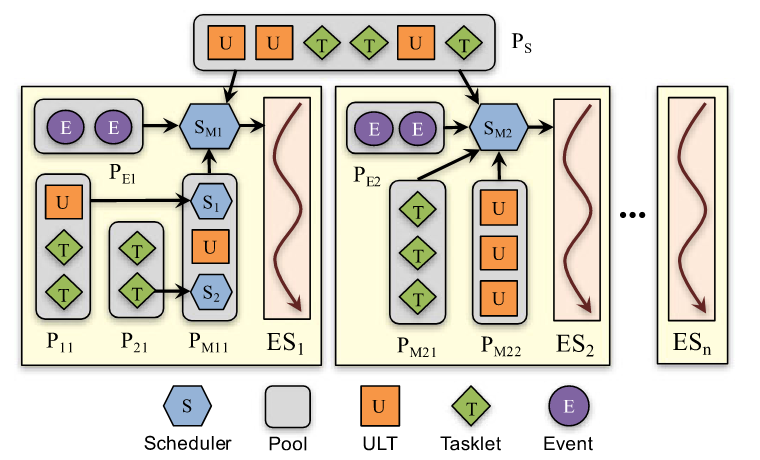
\includegraphics[width=0.8\linewidth]{res/argobot_application.png}
    \caption{Argobots execution model.}
    \label{fig:argobot-app}
\end{figure}

\begin{figure}[H]
    \centering
    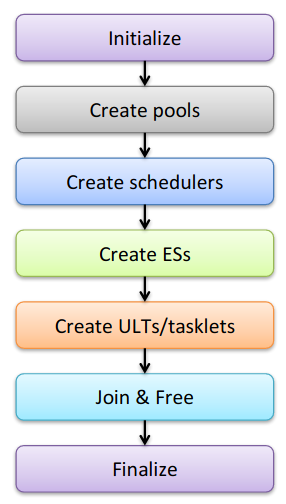
\includegraphics[width=0.35\linewidth]{res/control-flow.png}
    \caption{Argobots application flow of execution.}
    \label{fig:ex-flow}
\end{figure}

\subsection{Building blocks}
\subsubsection{Execution Streams}
Executions streams represents a sequential and independent instruction stream, which can consist of one or multiple non-preemptive work units (namely, ULTs and tasklets), it is mapped to a Pthread and can be bound to a hardware processing element such as CPU core or hardware thread. The work units to be executed are contained in one (or more) pools, and they are retrieved from one (or more) schedulers. Scheduling policies can be tweaked during runtime, and they determine the order in which work units flow to the execution stream and are thereby executed sequentially.\newline

Given the sequential nature of an ES, work units which are executed by the same ES do not require expensive synchronization mechanisms, since they do not run concurrently. However, synchronization is needed between work units executed in different ES running in parallel. 

\subsubsection{Schedulers}
Schedulers are responsible to deliver work units to the ES they are associated with, and they can implement different scheduling policies, which determines how work units are retrieved from pools and handled to the ES. Schedulers can be composed and scheduled just like work units, in order to compose different scheduling approaches dynamically, related to the computation at hand. Since a scheduler is considered as a work unit, it can be inserted into a pool and executed, which translates in a change of scheduling policy for the ES in charge, which will shift back to its original scheduler when the computation associated with the current scheduler is over.

\subsubsection{ULTs and Tasklets}
User-level threads and tasklets, also called \textit{work units}, represent two different types of workflow. User-level threads are independent execution units, which are executed in user space and can yield control to the scheduler, they can be dynamically migrated on a different execution stream during execution, since they have a private stack and context-saving capabilities. Tasklets, on the other hand, are considered to be ``lighter'' than ULTs, since they do not incur in costs related to context saving and stack management. They should be considered as atomic units of execution, which can't yield to a different execution and run to completion without context switching or suspension. 

\subsubsection{Pools}
Pools are containers of work units, and their sole purpose is to act as a uniform way of associating work to ES, indirectly, through schedulers. The only property associated with pools is the one regarding access, which can be set as private or shared. Shared pools may be used to implement a ``work-stealing'' strategy between two or more ESs. Pools are also used internally by the ES to receive asynchronous events.\newline

A pool associated with a running or stacked scheduler defines a set of work units ready to execute, which have to be controlled by the application programmer, since Argobots does not implicitly defines dependencies between work units. Hence, synchronization mechanisms offered by the library must be used to control the control flow of different work units.  Various operations can be performed over pools, like migration of work units to or from a specified pool, creation, destruction, and of course pop and push operations.

\subsection{Operations}
Argobots defines a set of operations which are common to all work units, made exception for some of them which are not available to Tasklets, given their execution model limitations. Implemented operations refer to:
\begin{itemize}
    \item Creation: allows the creation of work units, which are then inserted in a specific pool in a ready state. The type of pool and the associated scheduler(s) will determine the time and context of execution;
    \item Join: work units can be joined by other ULTs, which wait for their termination;
    \item Yield: a work unit can cooperatively yield control to the scheduler which is executing in the current ES at the time of yielding. The scheduler will then gather the next work unit to be executed following the implemented policy;
    \item Yield\_to: a ULT can decide to yield control to a specific ULT in the same ES. This operation avoids the overhead of one context switch by bypassing the scheduler;
    \item Migration: allows work units to be migrated between pools;
    \item Synchronization: ULT can rely over usual synchronization mechanisms implemented by Argobots, such as mutexes, condition variables etc.
\end{itemize}

\subsection{Memory Management}
Argobots is intended to be used in fine-grained dynamic environments, where creation and destruction of work units, as well as context switch between them, take place at high frequencies.\newline

Since, as shown in \cite{argobots-paper}, memory allocation and deallocation contribute to most of the time required to create and destroy a work unit, Argobots developed its own memory allocator. The memory allocator creates, for each ES, a memory pool which is subsequently used to manage all creation and destruction calls of work units. The memory pool is held private per ES, in order to avoid heap access synchronization upon creation of work units by means of the same ES. The size of the pool is tied to the number of work units which are spawned and allows to return memory to the system upon their destruction, if the pool reached a given threshold.\newline

Context switching, on the other hand, has a lower cost in terms of memory, compared to creation and destruction of work units, and it is only related to ULTs, since tasklets are atomic operations and can't yield to other work units. Context switching costs are mostly associated with:
\begin{itemize}
    \item ULT suspension: context of the currently running ULT must be saved and context of the next ULT must be resumed. However, the first step can be avoided if the yielding ULT is terminating and will not be resumed later;
    \item ULT join: the join operation suspends the caller and yield control to the scheduler, until the joined ULT terminates its execution. However, if two ULTs are in the same ES, the joining ULT can directly yield control to the joined ULT, bypassing the context switch to the scheduler entity.
\end{itemize}

% \subsection{Mixing Argobots with standard library threads}
% During the testing phase, we analyzed but still not tracked down an annoying drawback of mixing up two threading environments together. FastFlow uses standard library thread calls to run each node in a different thread, instead Argobots internally creates its own thread-mapped execution streams upon initialization, and associates a ``primary'' execution stream to the 
\chapter{Margo}
\label{sec:margo}
Margo \cite{mochi-core} is a Mercury binding that uses Argobots as a runtime library. Just like Mercury, Margo requires both origin and target nodes to register for RPC calls associated with a specific identifier (a string) and an input/output type, which must necessarily be registered using the relative macros, as we describe in the following.\newline
By using Argobots as a runtime library, Margo hides the handling of Mercury's progress loop by delegating it to a specific Argobots ES (namely, a physical thread). Moreover, Margo allows to freely manage how the various RPC associated callbacks will be dispatched among internal pools and external user defined pools. When initializing Margo, the user can specify its own pools and ESs that will be responsible for both progress loop and RPC calls, otherwise the programmer can decide to completely let Margo handle the calls with its own pools and ESs.\newline

Being a binding between Mercury and Argobots, Margo retains all the concepts we defined in the previous section, however, Margo greatly simplifies the development of RPC-based services by introducing extensions to the Mercury-based model:
\begin{itemize}
    \item more intuitive communication: Margo defines wrappers based on Argobots runtime in order to present asynchronous communication mechanisms as a user-level thread communication model. Communication facilities are handled by ULTs, which can be suspended and resumed as communication proceeds;
    \item progress loop abstraction: polling and communication events are internally managed by a ULT. Policies for handling RPC-related execution can be manually defined and tweaked to better suit the application needs. In this way, multiple providers can be easily handled and multiplexed by the same core process, without the need of handling multiple progress loops at once;
    \item renewed polling strategy: Margo allows both busy and idle mode, which allows to tweak Margo for both performance and resource consumption needs.
\end{itemize}
\section{RPC registration process}
\label{sec:rpc-reg}
In this section we describe the RPC registration process, which follows a standardized procedure and requires RPC input and output types, as well as routines to pack the types into network buffers, to be defined by both origin and target nodes. Additionally, the callback function to be executed must be defined by the target node with a predefined signature in order for Margo to encapsulate it in the internal service functions which triggers RPC execution upon receiving the request from the origin node.\newline

The registration process must proceed by:
\begin{itemize}
    \item defining input and output types: as shown in \hr{type-rpc}{Listing}, RPC arguments types must be defined by the means of a C-style \texttt{struct} datatype, which can internally contain all the necessary types for the RPC call;
    \item defining the packing routine: \hr{packing-routine}{Listing} defines the routine which is internally used by Margo to correctly write to and read from the network buffers which are then used to send and receive RPC data arguments. Margo also offers a ``simplified'' way of defining such routines, which we omit for sake of presentation and to better explain how the internal network buffers are built and filled with data. Each packing routine is strictly tied to a specific type. Having a type \texttt{X}, the routine must be defined as \texttt{hg\_proc\_X}, and it must encode and decode each of the field contained in the \texttt{X} struct type. Additionally, Margo can be built with XDR capabilities which will in turn change the way data are represented in the buffer exchanged between nodes, however, since FastFlow distributed version shares already serialized streams, we don't rely upon this functionality.
    \item defining the actual RPC callback: this step is only required by the node which will act as a ``server'' for the specific RPC. In \hr{rpc-def}{Listing} we provide a sample RPC callback declaration and definition, which allows the server node to define the function to be executed upon an RPC request from another node. RPC callback declaration and definition require also a call to specific macros defined by Margo, which will wrap the RPC callback defined by the user with Argobots-aware code, necessary for Margo to dispatch RPC callbacks among different ULTs.
    \item associating an ID to the RPC: after having registered all the types and routines, both origin and target nodes have to associate a common ID for the RPC that they intend to use. This can be done as shown in Listings \textbf{\ref{margo-register-origin}} and \textbf{\ref{margo-register-target}}. The registering process is complete, and the origin node can now use the returned RPC identifier to issue requests to the listening target node by using a \texttt{margo\_forward} call. Note that, after the registration process is complete, the listening node can receive RPCs calls with the specified ID from all the origin nodes which registered an RPC with the same ID.  
\end{itemize}


\noindent\begin{minipage}{.40\textwidth}
\begin{lstlisting}[caption=RPC type definition.,language=C++, style=mystyle, label=type-rpc]{type-rpc}
typedef struct {
    hg_int64_t   hash_val;
    hg_uint64_t  size;
    hg_bulk_t    bulk_handle;
} ff_rpc_in_t;
\end{lstlisting}
\end{minipage}\hfill
\begin{minipage}{.48\textwidth}
\begin{lstlisting}[caption=Packing routine definition. Allows the Margo framework to manage data from/to the network buffer used internally to ship data during RPC calls. Each of the type-specific routines allows data copies which are aware of the size of data to be packed/unpacked.,language=C++, style=mystyle, label=packing-routine]{packing-routine}
hg_return_t
hg_proc_ff_rpc_in_bulk_t(hg_proc_t proc,
                         void* data) {
    
    ...
    // Retrieve input data structure
    ff_rpc_in_t* in = (ff_rpc_in_t*)data;

    // Write/read data to/from Margo's
    // send/receive buffer carried by `proc'
    hg_proc_hg_int64_t(proc,
            &in->hash_val);

    // We call a specific routine for each
    // field in the RPC input struct
    hg_proc_hg_uint64_t(proc,
            &in->size);

    hg_proc_hg_bulk_t(proc,
            &in->bulk_handle);

    ...
}
\end{lstlisting}
\end{minipage}
\begin{center}
\vspace{-0.1cm}
\begin{minipage}{0.55\textwidth}
\begin{lstlisting}[caption=RPC declaration and definition,language=C++, style=mystyle, label=rpc-def]{rpc-def}
void ff_rpc(hg_handle_t handle);
DECLARE_MARGO_RPC_HANDLER(ff_rpc);

void ff_rpc(hg_handle_t handle) {
    ff_rpc_in_t           in;
    const struct hg_info* hgi;
    margo_instance_id     mid;

    // Get input data
    margo_get_input(handle, &in);
    
    // Retrieve objects to identify current RPC
    // and get back registered data
    hgi = margo_get_info(handle);
    mid = margo_hg_info_get_instance(hgi);

    // Here data may be retrieved and used
    // internally in the RPC call

    margo_free_input(handle, &in);
    return;
}
DEFINE_MARGO_RPC_HANDLER(ff_rpc)
\end{lstlisting}
\end{minipage}
\end{center}

\begin{center}

\begin{minipage}{.65\textwidth}
\begin{lstlisting}[caption=Finalization of the registration process in the origin node. The register macro specifies the input/output expected types as well as the packing routines as described above.,language=C++, style=mystyle, label=margo-register-origin]{margo-register-origin}
int main(int argc, char** argv) {
    // Margo initialization code
    ...

    // Initialize the Margo instance used to perform
    // Margo-related calls
    margo_instance_id mid;
    mid = margo_init(listening_addr, MARGO_CLIENT_MODE, 1, 1);
    ...
    my_rpc_id = MARGO_REGISTER(mid, "ff_rpc",
                    ff_rpc_in_t, ff_rpc_out_t, NULL);
    
    // Looks up for a server 
    hg_addr_t svr_addr;
    margo_addr_lookup(mid,
                    svr_addr_str, &svr_addr);
    
    // Creates the handle for the RPC call
    hg_handle_t handle;
    margo_create(mid, svr_addr,
                    my_rpc_shutdown_id, &handle);
    margo_forward(handle, NULL);
    ...
}
\end{lstlisting}
\end{minipage}
\end{center}

\begin{center}
\vspace{-0.1cm}
\begin{minipage}{.65\textwidth}
\begin{lstlisting}[caption={Finalization of the registration process in the target node. The listening node only needs to register the RPC types and routines, as the origin node, and additionally it needs to specify the RPC callback for the registered ID.},language=C++, style=mystyle, label=margo-register-target]{margo-register-target}
int main(int argc, char** argv) {
    // Margo initialization code
    ...

    // Initialize the Margo instance used to perform
    // Margo-related calls
    margo_instance_id mid;
    mid = margo_init(protocol, MARGO_SERVER_MODE, 1, 1);
    my_rpc_id = MARGO_REGISTER(mid, "ff_rpc",
                    ff_rpc_in_t, ff_rpc_out_t, ff_rpc);
    
    margo_wait_for_finalize(mid);
}
\end{lstlisting}
\end{minipage}
\end{center}

\section{Margo analysis}
As we pointed out in \S\ref{sec:mercury-analysis}, most of the limitations are tied to the support of the various plugins and their functionalities. Margo, besides sharing all these limitations, introduce an incredibly easy interface to implement multi-homed RPC services, which greatly simplifies the development of RPC-based FastFlow nodes.\newline

The main limitation of the Margo library are mostly related to how RPC calls are handled, in particular with reference to data copies happening between the input data and the send/receive buffers used to ship RPC data through the network. However, further investigation is needed at this point in time to analyze how those limitations can be avoided, without relying on the bulk functionalities, which however remain a suitable fallback method if data copies are unavoidable. However, a further problem is introduced in the utilization of bulk transfers via RDMA where no responses are expected from the sender, in fact in this particular case one must be extremely careful about freeing memory that has still not been read from the remote end.\newline

Margo, on its hand, introduces additional dependencies which are related to the libraries it uses in the underlying layers and how it handles configuration strings. The introduced dependencies are the following:
\begin{itemize}
    \item Mercury: as described in \S\ref{sec:mercury}, in particular requires for this framework to be built with \ttt{-DMERCURY\_USE\_SYSTEM\_BOOST:BOOL=OFF -DMERCURY\_USE\_BOOST\_PP:BOOL=ON}, which enable pre-processors macro in Mercury in case BOOST library is not present in the system. Since we do not want to be dependend on BOOST library, this is necessary since Margo uses these macros internally;
    \item Argobots: as described in \S\ref{sec:argobots};
    \item json-c: A JSON implementation for C language\cite{jsonc}, needed internally by Margo in order to generate configurations based on json-formatted strings provided at initialization of Margo instances.
\end{itemize}
\chapter{Implementation}
\label{sec:implementation}
\section{Communication classes}
We developed FastFlow's communication classes by extending the \ttt{ff\_node\_t} class, in such a way the developed classes can be used in any context where a \ttt{ff\_node\_t} can be used. However, we show that they naturally sit at the extremes of a pipeline building block, since they offer functionalities to receive and forward data from and through the network.\newline

The classes we implemented are strictly tied to the concepts of receiver and sender node, and they make use of Margo's capabilities of developing multi-endpoint services without requiring to manually handling progress loops. At the current stage of development, there is no personalized behaviour based on the endpoint which received a call to the registered RPCs. This represents the next main step in the evolution of the implemented classes. (De)Multiplexing, however, should be fairly easy to handle thanks to the internal mechanisms that Margo offers in order to identify the origin node which issued a request. Having personalized behaviour, depending on the specific endpoint, is very important to deal with the grouping concept introduced since the distributed version of FastFlow has been developed. Particularly pathological cases, where a personalized behaviour must be implemented given the specific endpoint on which the request is received, benefit from the automatized mechanisms offered by Margo. Moreover, the simplicity in handling multiple endpoints via the implemented classes allow to test a multitude of situations with little to no code changes.\newline

\subsection{Receiver node}
Receiver node is a FastFlow \texttt{ff\_node\_t} that relies on a Margo instance initialized with \texttt{MARGO\_SERVER\_MODE}. This allows the receiver node to wait for incoming RPC requests at the specified addresses. A list of addresses can be provided at initialization, translating in a receiver node listening for the same set of RPC functionalities on all of the provided endpoints. \hr{receiver-skeleton}{Listing} shows pseudo-code of the implemented receiver node.
\begin{lstlisting}[language=C++, style=mystyle, caption={Receiver node pseudo-code.}, label={receiver-skeleton}]{receiver-skeleton}
struct receiverStage: ff_node_t<Task> {
    std::vector<margo_instance_id> mids // Margo instances to be used during servicing

    // Parametrized constructor which registers all specified endpoints with the
    // provided configuration strings.
    receiverStage(std::array<char*> endpoints, std::array<char*> configs) {
        ...
        for(i < num_endpoints) {
            // init_endpoint initializes a Margo server instance on the provided address
            // and config string. The endpoint allocates a specific ES and pool to handle
            // all the requests coming through the specified address.
            // Returns an handle to the created Margo instance
            mids[i] = init_endpoint(endpoints[i], configs[i]);
            
            // Code to get the end address (to be forwarded and used by the sender node)
            // and various debugging can be put here, by using the mids generate by the init
            // phase
            ...
            
            // Use the initialized mids to register the set of RPCs that will be offered by
            // this receiver node.
            // Responses for the registered RPCs are disabled.
            register_service(mids[i])
        }
    
    }
    
    // The receiver node has nothing to do in the service method, it can simply wait
    // for termination of all the listening endpoints and forward the EOS at the end.
    // `task' parameter is ignored in this stage, since it acts as a sort of `endo-stream'
    // generator for the other stages in the pipe.
    Task* svc(Task* task) {
        wait_for_finalize(mids);
        return EOS;
    }
}
\end{lstlisting}

\subsection{Sender node}
Sender node, on the other hand, relies over Margo instance initialized with \texttt{MARGO\_CLIENT\_MODE}, since we do not expect this node to be listening on any RPC request for now.  The current version of the sender node allows to contact only a single endpoint at a given address. The address to contact for this specific node must be provided at initialization, and at the moment it is not possible to change the remote service address. In the next versions the possibility to contact multiple addresses, in order to implement the pathological grouping case described before, will be implemented following the same approach used for the receiver stage. Pseudo-code for this class is provided in \hr{sender-skeleton}{Listing}.

\begin{lstlisting}[language=C++, style=mystyle, caption={Sender node pseudo-code.}, label={sender-skeleton}]{sender-skeleton}
struct senderStage: ff_node_t<Task> {
    margo_instance_id       mid;        // Margo object to use for communications
    hg_addr_t               svr_addr;   // Server address listening for incoming RPCs

    senderStage(char* addr) {
        // Initialize the Margo instance as a client node and creates the necessary
        // objects to register RPC calls and addresses to issue the requests to the
        // specified address.
        mid = init_endpoint(addr);
        
        // This is the exact same function that is called by the receiver, but in this
        // case we don't need to provide implementation of the actual RPC function.
        register_service(mid);
    }

    Task* svc(Task* task) {
        // The task received by the previous stage is packed into the RPC registered
        // type and forwarded to the sender via an RPC call. The current node can
        // proceed since no response is expected.
        ff_rpc_in in = pack_task(task);
        forward_task(mid, in);
        return GO_ON;
    }

    void svc_end() {
        // Upon termination forwards a shutdown RPC to the connected receiver node.
        // The sender has nothing to do more than cleaning Margo resources. 
        forward_shutdown(mid, shutdown_id);
        finalize(mid);
    }
};
\end{lstlisting}

\section{RPC based service}
The developed classes allow distributed groups to communicate through a fixed set of RPC calls, which are shared among receiver and sender nodes and used for all the communications between the various groups. Two RPCs are offered by the communication service, and they refer to:
\begin{itemize}
    \item \texttt{ff\_rpc}: this RPC is used during the whole lifetime of the FastFlow application, and it is used by the sender node, upon reception of a stream element, to forward the current stream element to the receiver node it is connected to. The sender node packs the data in the RPC input type, as described in \textbf{\S\ref{sec:rpc-reg}}, and ships them issuing a forward call to the connected endpoint. Since no response is expected from the RPC call, the sender can proceed immediately.
    \item \texttt{ff\_rpc\_shutdown}: this RPC is only used upon reception of an EOS object from the stream. In this case no data needs to be sent through the network, but only a signal that the stream has ended, in order to allow the receiving node to gracefully terminate its execution and forward EOS accordingly to the local group's nodes. Signaling an EOS propagates through the network, since the receiver node will generate an actual EOS object when the \texttt{ff\_rpc\_shutdown} callback is executed that will allow local nodes to terminate as per FastFlow's execution flow. At that point, the next sender node will issue an end-of-stream RPC and the whole FastFlow application will terminate. Note, however, that a receiver node will not forward an EOS object unless all the listening endpoints have received a shutdown RPC.
\end{itemize}

It is important to point out that this set of RPC callbacks need to be registered only once per Margo instance. This means that, once for each listening endpoint, the receiver node must register the same set of RPCs, but it is completely agnostic on the number of nodes that will issue RPC requests on the same endpoint. 

\section{Splitting taxonomy}
In this section we analyze the characteristics of different connections that take place between remotely connected groups, we show that very specific types can be determined whether the splitting happens in a \textit{horizontal} or \textit{vertical} fashion. We describe the specific categories depending on different splitting strategies. To better explain the identified categories, we introduce the concepts of \textit{level}, \textit{horizontal} and \textit{vertical} splits. Considering a generic FastFlow application as a pipeline of stages, we naturally associate a \textit{level} to each stage incrementally. In addition, we define as \textit{horizontal} a split which creates two groups sitting at the same level of the original pipeline, instead we define as \textit{vertical} a split which creates groups operating at two different levels of the pipeline. Note, however, that a \textit{vertical} split can internally contain further \textit{vertical} or \textit{horizontal} splits. Given these definitions, we can identify two categories that describe each of the connections in remotely-connected groups, specifically:
\begin{itemize}
    \item \textit{internal}: elements to be sent/received are related to a connection that takes place between groups that are split horizontally. Connections of this type can be linked to splittings that divides an original FastFlow building block in two groups belonging to the same pipeline level, for example an \textit{all-to-all} building block divided by distributing left and right workers in two groups;
    \item \textit{external}: elements to be sent/received are related to connections that take place between two groups at different levels of the original pipeline. These connections are typically related to vertical splits of the original FastFlow application.
\end{itemize}

To better illustrate this taxonomy, we present a simple example which contains every concept we introduced up to now. In \hr{fig:original-a2a}{Figure} there is a sample FastFlow application composed of an \textit{all-to-all} building block with two left workers and two right workers. By performing an \textit{horizontal} ``cut'', we want to split the \textit{all-to-all} in two different groups, each of them with one left worker and one right worker. If we consider this \textit{all-to-all} block to be in the middle of a pipeline, the groups will finally be as depicted in \hr{fig:taxonomy}{Figure}. We show the structure of the main software entities that handle the splitting. As we can see, the amount of nodes participating in the application increases to facilitate communication between remote groups, both via \textit{internal} connections (LS1 to RS2) and via \textit{external} ones (ff\_receiver to LS2).\newline

We will proceed now by describing the bigger picture by delving into particulars and explaining each of the involved parts and messy communication lines. The reasoning is very simple once the way communications are handled is clear, but it can seem pretty complicated at the start. We depicted in different colours the data flow which involve a stream element as the same ``origin'' object. When the colour of a communication line changes, also the provenance attached to the considered object will change. We describe in the following the different concepts depicted in the picture below:
\begin{itemize}
	\item left/right box: they are abstracted representations of \textit{internal} nodes in remotely connected groups. Left and right boxes of horizontally split groups, belonging to the same original building block, are logically connected by mean of their own local sender and receiver nodes. Since they respectively emulate a left and right worker, a stream element received by a left box (and hence originally shipped by a right box in a remote group) will be forwarded to a right worker in the current local group.
	\item red channel: carries stream elements which are part of the normal flow of execution, for example streaming elements flowing through the stage of a pipeline one after the other.
	\item purple/green channel: represents \textit{internal} connection channels.  They allow communication between boxes of different groups in order to maintain the \textit{all-to-all} semantic in a distributed environment.
\end{itemize}

The connections, internally, are determined by each remote group by means of the configuration file provided upon initialization and by the information that are exchanged during the startup phase. In this way, each receiver/sender node can associate correctly the ID of each channel to the various entities that are created after the splitting is performed.

\begin{figure}[H]
	\centering
	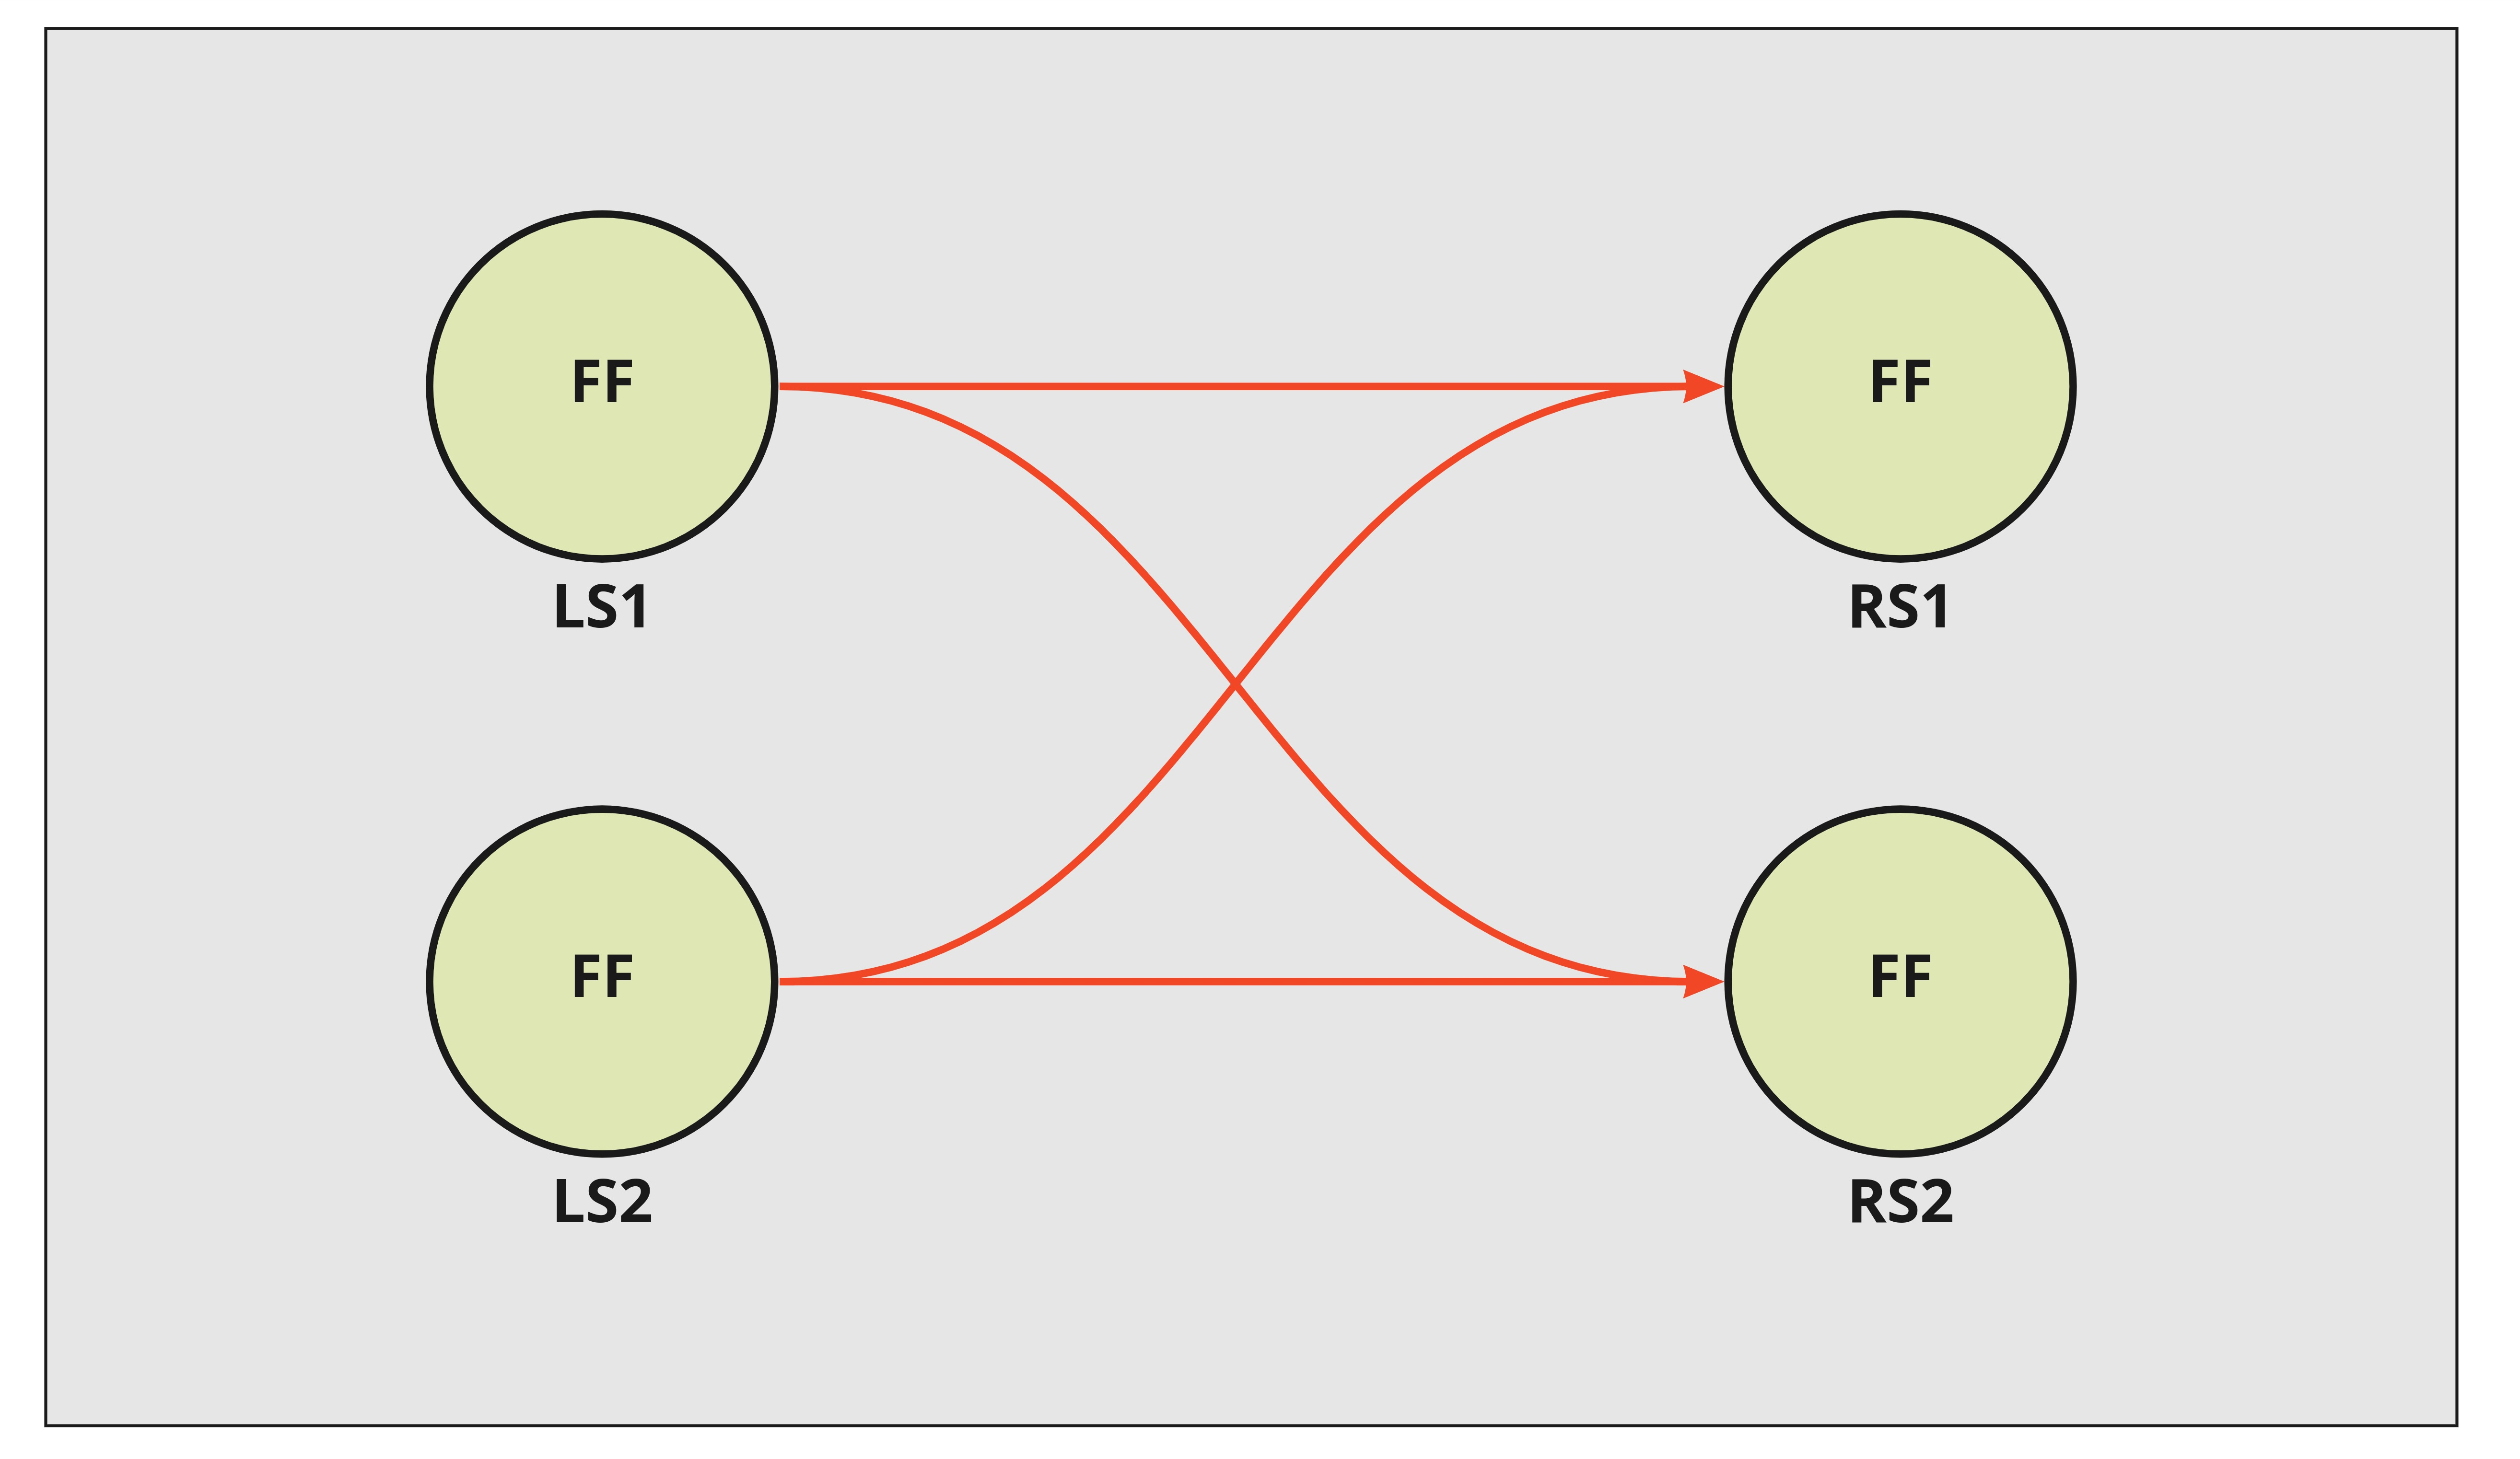
\includegraphics[width=0.5\linewidth]{res/original-a2a.jpg}
	\caption{Sample A2A building block.}
	\label{fig:original-a2a}
\end{figure}

\begin{figure}[H]
    \centering
    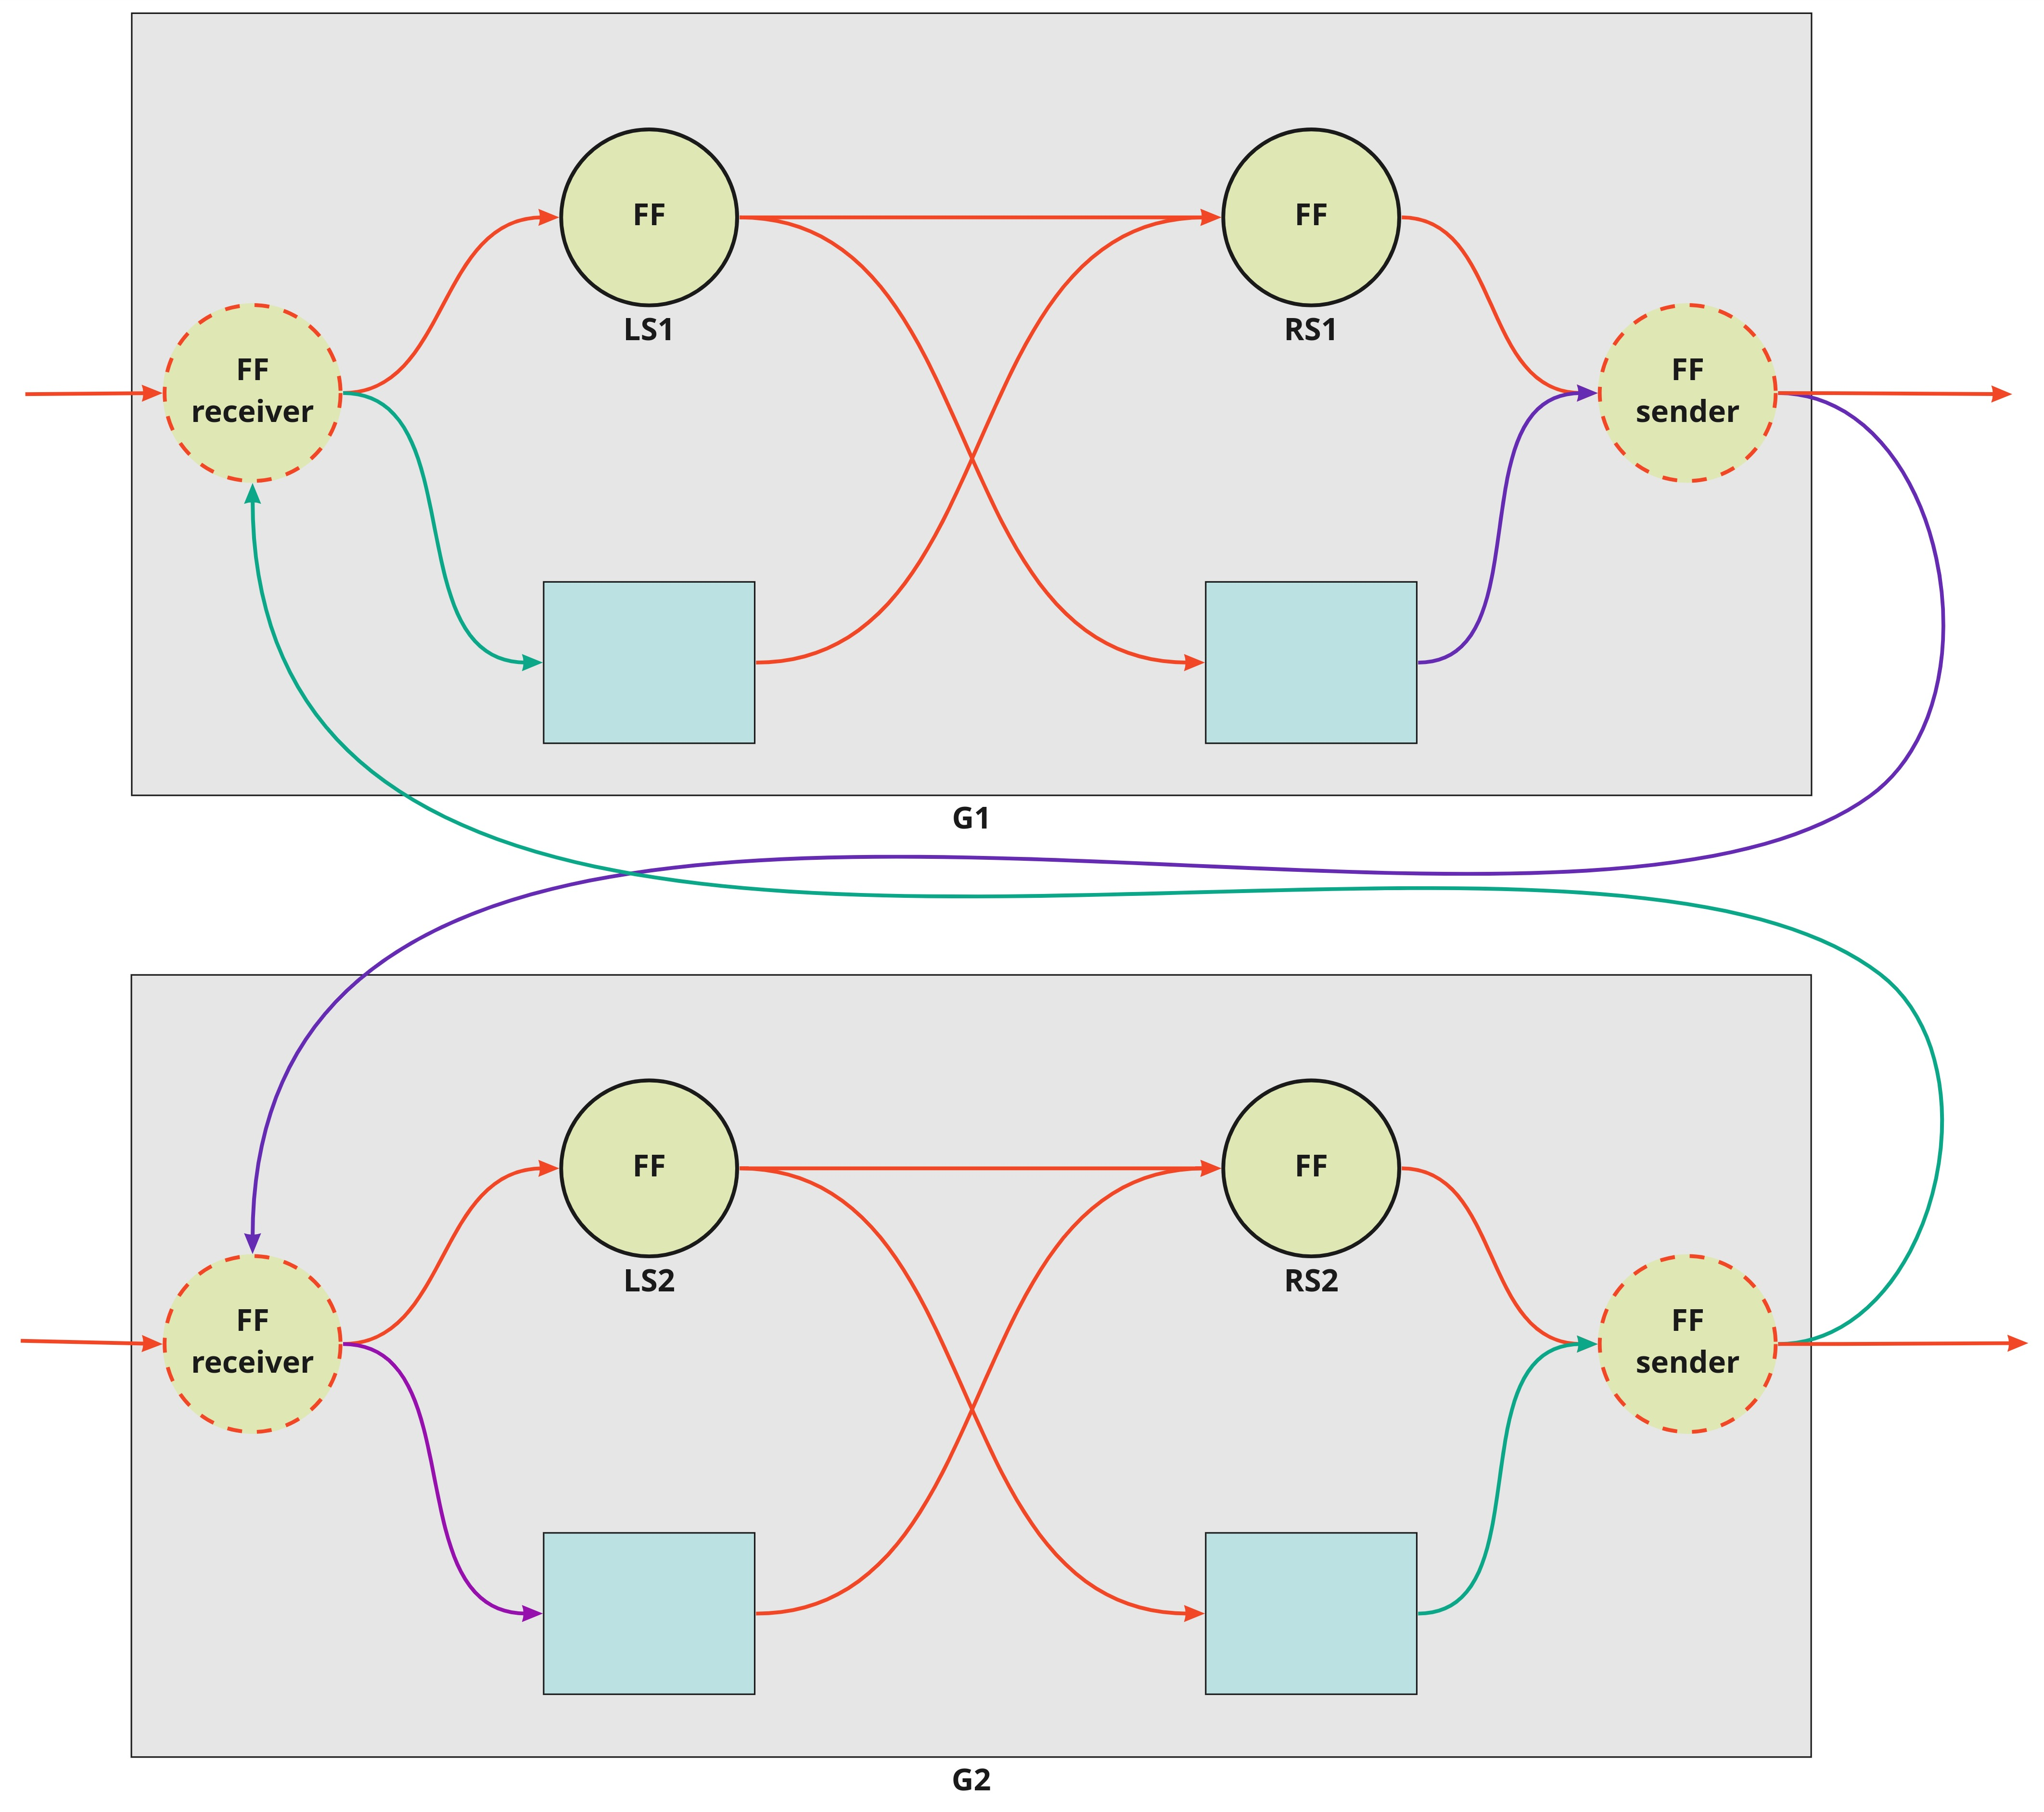
\includegraphics[width=0.8\linewidth]{res/taxonomy.jpg}
    \caption{Pathological case representing the splitting of an A2A node into two groups which needs to communicate internally in order to retain the original semantic of the A2A building block.}
    \label{fig:taxonomy}
\end{figure}
\section{Testing}
\label{sec:testing}
In this section we show the testing application we have developed to assess the functionalities of the implemented classes described in \S\ref{sec:implementation}.

\subsection{A sample application}
In \hyperref[fig:sample-app]{\textbf{Figure \ref{fig:sample-app}}} we show a sample application developed to test the implemented classes for communication. As it can be seen, the structure of the application is very simple, we have three groups communicating in a pipeline fashion, by means of implemented \texttt{sender} and \texttt{receiver} nodes. Communication between groups can happen with the different plugins provided by the Mercury library, and switching from one plugin (transport) to another is only a matter of passing as configuration string the desired plugin (transport) to use for communication.\newline

\hr{fig:node-legends}{Figure} shows the legend for the nodes and communication channels used in the sample application. We have two types of nodes, sequential ones which are standard \ttt{ff\_node\_t}, and Margo-injected nodes which are used for communication between distributed groups. Simple plain arrows indicates usual FastFlow shared memory channel, instead bullet-tailed arrows indicate a distributed connection between two nodes. Note, however, that ``distributed'' here only means that two groups are connected through Margo calls, but the nodes can reside in the same machine and communicate with the shared memory plugin provided by Margo, as it happened in part of the testing phase.

\begin{figure}[H]
    \centering
    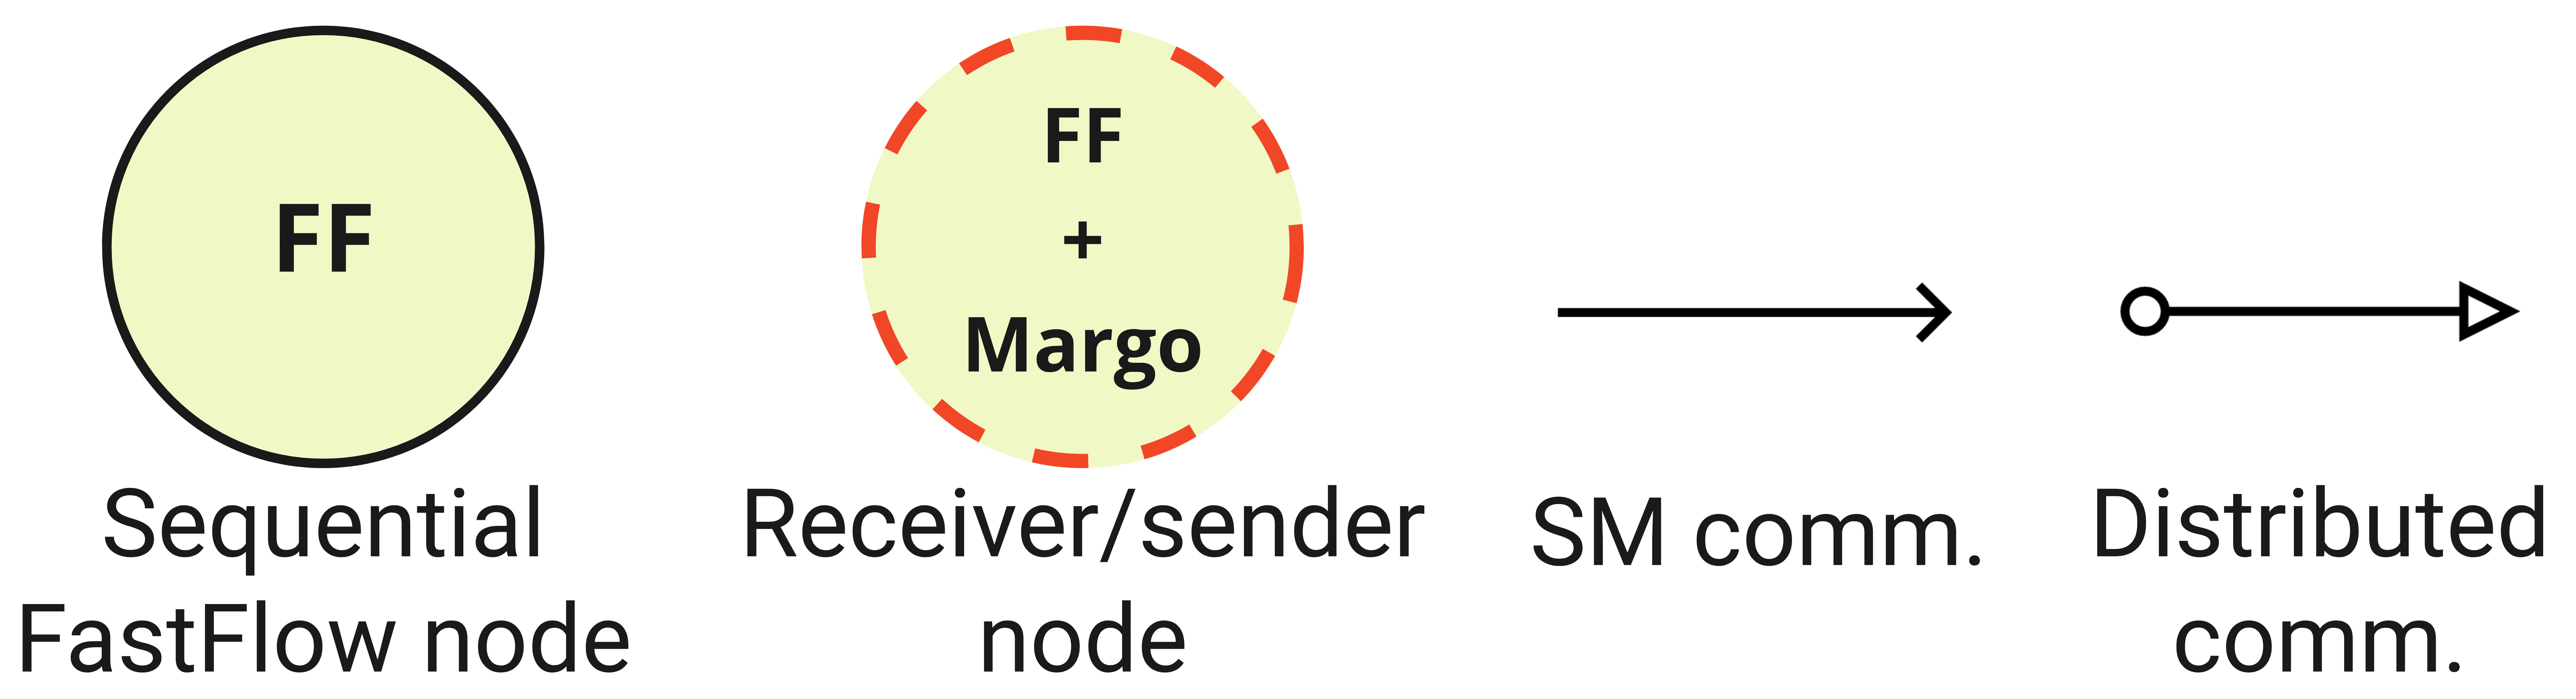
\includegraphics[width=0.6\linewidth]{res/node-legends.jpg}
    \caption{Node legends}
    \label{fig:node-legends}
\end{figure}
\begin{figure}[H]
    \centering
    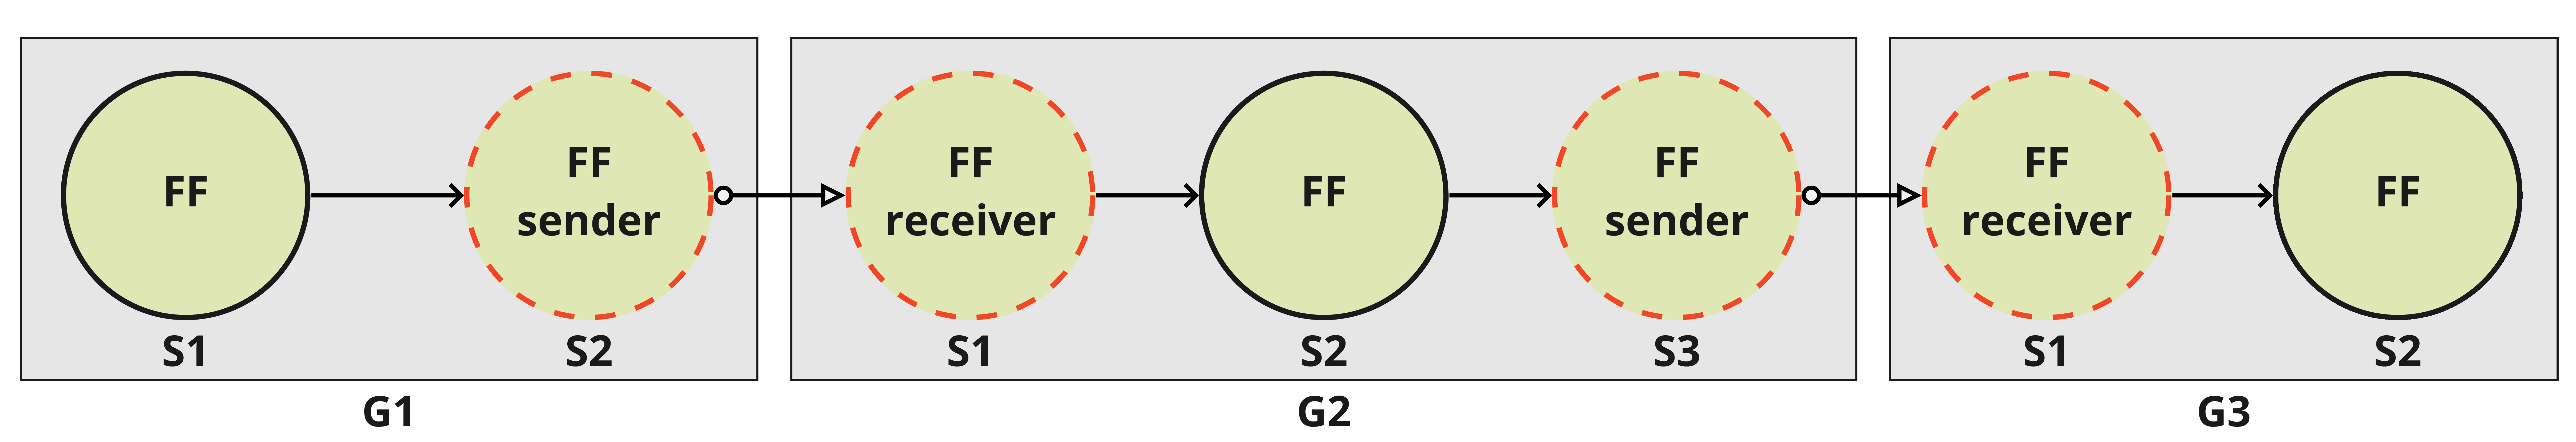
\includegraphics[width=\linewidth]{res/sample-app.jpg}
    \caption{A sample testing application composed of three main groups which are connected by using the implemented classes using Margo library.}
    \label{fig:sample-app}
\end{figure}

Moreover, the standard FastFlow nodes depicted in \hr{fig:sample-app}{Figure} can be any composition of standard FastFlow building blocks. We showed here, for simplicity, a single sequential \ttt{ff\_node\_t}. The important thing to notice is that \ttt{sender} and \ttt{receiver} nodes are mandatory, respectively as last and first nodes, in order to compose distributed groups correctly. The depicted groups represents, potentially, the three situations that may occur when splitting a standard FastFlow application in a distributed one, that are:
\begin{itemize}
    \item (G1): group with only out remote connections. In this case only a \ttt{senderStage} is needed as a last node in the application pipeline. The pipeline is most likely to generate elements from an endo/eso-stream;
    \item (G2): group with both in/out remote connections. Both \ttt{receiverStage} and \ttt{senderStage} are needed, respectively as first and last nodes in the pipeline. All internal nodes receive and send stream elements using Margo-injected nodes;
    \item (G3): group with only in remote connections. Only a first \ttt{receiverStage} pipeline node needed.
\end{itemize}

In \hr{FFMargo-skeleton}{Listings}, we show a skeleton with required library calls necessary to initialize Margo and Argobots environment, which are necessary steps before composing FastFlow building blocks with the implemented communication nodes.

\begin{lstlisting}[language=C++, style=mystyle, caption={Skeleton of a sample FastFlow application using Margo as communication layer.}, label={FFMargo-skeleton}]{FFMargo-skeleton}
int main(int argc, char** argv)
{
    ...

    // Setting up main Argobots instance
    margo_set_environment(NULL);
    ABT_init(0, NULL);

    {
        // Here we place code to build each of the groups composing
        // the application, namely G1, G2, G3.
    }

    // Finalizing Argobots
    ABT_finalize();
}
\end{lstlisting}

After having initialized the environment with the required library calls, we proceed by building the groups that have to be executed as follows:
\begin{itemize}
    \item group G1: implemented in \hyperref[G1-node]{\textbf{Listing \ref{G1-node}}}, creates two nodes, the first one is a simple FastFlow \texttt{ff\_node\_t} generating a stream of elements to forward to other nodes, the second one is a \texttt{senderStage} initialized with the address of the \texttt{receiverStage} to which elements will be forwarded using the Margo communication mechanisms;
    \item group G2: implemented in \hr{G2-node}{Listing}, builds three stages, where the first and the last one are communicator nodes, respectively a \ttt{receiverStage} and a \ttt{senderStage}. The middle node is a simple \ttt{ff\_node\_t} which simply lets tasks flow between the two nodes communicating with groups G1 and G3;
    \item group G3: implemented in \hr{G3-node}{Listing}, builds a \ttt{receiverStage} and a standard \ttt{ff\_node\_t} node which simply prints the tasks received.
\end{itemize}

\begin{center}
\begin{minipage}{.45\textwidth}
\begin{lstlisting}[caption=G1 node composition,language=C++, style=mystyle, label=G1-node]{G1-code}
firstStage  first(stream_len);
senderStage sender(receiver_addr);
ff_Pipe<float> pipe(first, sender);
if (pipe.run_and_wait_end()<0) {
    error("running pipe");
    return -1;
}
\end{lstlisting}
\end{minipage}\hfill    
\end{center}

\begin{center}
\begin{minipage}{.63\textwidth}
\begin{lstlisting}[caption=G2 node composition,language=C++, style=mystyle, label=G2-node]{G2-code}
// Build addresses vector
...

receiverStage receiver(addresses);
forwardStage first;
senderStage sender(receiver_addr);
ff_Pipe<float> pipe(receiver, first, sender);
if (pipe.run_and_wait_end()<0) {
    error("running pipe");
    return -1;
}
\end{lstlisting}
\end{minipage}
\end{center}

\begin{center}
\begin{minipage}{.63\textwidth}
\begin{lstlisting}[caption=G3 node composition,language=C++, style=mystyle, label=G3-node]{G3-code}
// Build the addresses vector
...

receiverStage receiver(addresses);
forwardStage first;
ff_Pipe<float> pipe(receiver, first);
if (pipe.run_and_wait_end()<0) {
    error("running pipe");
    return -1;
}
\end{lstlisting}
\end{minipage}
\end{center}

With the implemented classes, building various groups communicating between each other is very simple and straightforward. Moreover, the way communications are abstracted by the underlying frameworks, makes it easy and painless to extend functionalities of the communication nodes. Adding new protocols requires zero effort and no code modifications from the user point-of-view, since the only step to follow is to define a Mercury-accepted string with the preferred protocol to use during communication and use it at initialization of the receiver node.\newline

Note that, since the receiver stages can be initialized with a vector of strings which represents all the endpoints to which the receiver will listen on, we can (and we must, to allow correct termination) compose multiple instances of groups (G1) and (G2), based on the amount of endpoints created, respectively by (G2) and (G3). For example, if we create a group (G2) with two listening endpoints, in order to allow the whole application to terminate correctly, we must run two (G1) connecting, in turn, to both the endpoints.
\newpage

\printbibliography
\newpage
% \section*{Appendix A}
\label{sec:appendix}

% \listoftodos
\end{document}
